\newpage
\subsubsection{Die Kosinus Funktion}

\begin{itemize}
    \item $cos(deg(x))$
    \item diese Funktion hat eine Periode von $2*\pi$
\end{itemize}


\hfill \break
Die Wertetabelle und Graphik zu $cos(deg(x))$:\\
\fboxrule=0.8pt \fcolorbox{lightgray}{lightgray}{%
    \begin{tabular}{c|c}
        $x$               & $y$ \\
        \hline
        $0$               & 1   \\
        $\frac{\pi}{2}$   & 0   \\
        $\pi$             & -1   \\
        $\frac{3*\pi}{2}$ & 0  \\
        $2*\pi$           & 1   \\
    \end{tabular}}\\


\hfill \break
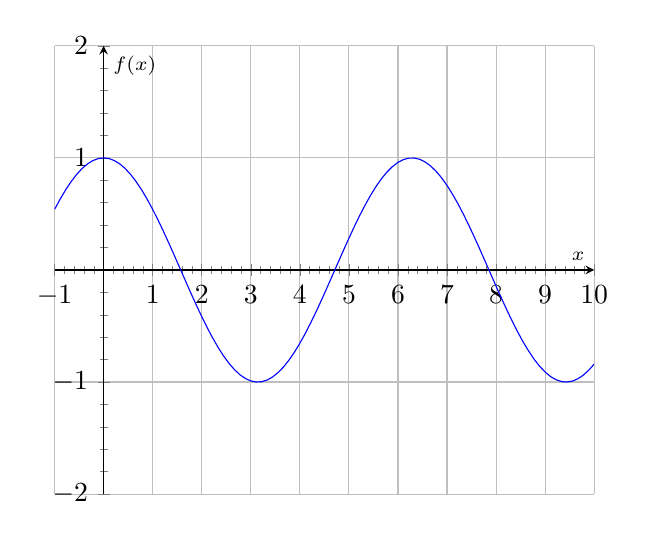
\begin{tikzpicture}[scale=1]
    \begin{axis}%
        [
            grid=major,
            xtick={-1,0,...,10},
            minor x tick num=4,
            xmin=-1,
            xmax=10,
            xlabel={\scriptsize $x$},
            axis x line=middle,
            ytick={-2,-4,...,2},
            minor y tick num=4,
            ymin=-2,
            ymax=2,
            ylabel={\scriptsize $f(x)$},
            axis y line=middle,
            no markers,
            samples=100,
            domain=-1:10,
        ]
        \addplot[blue] (x,{cos(deg(x))});
    \end{axis}
\end{tikzpicture}